\begin{figure*}[!htbp]
\begin{minipage}{6in}
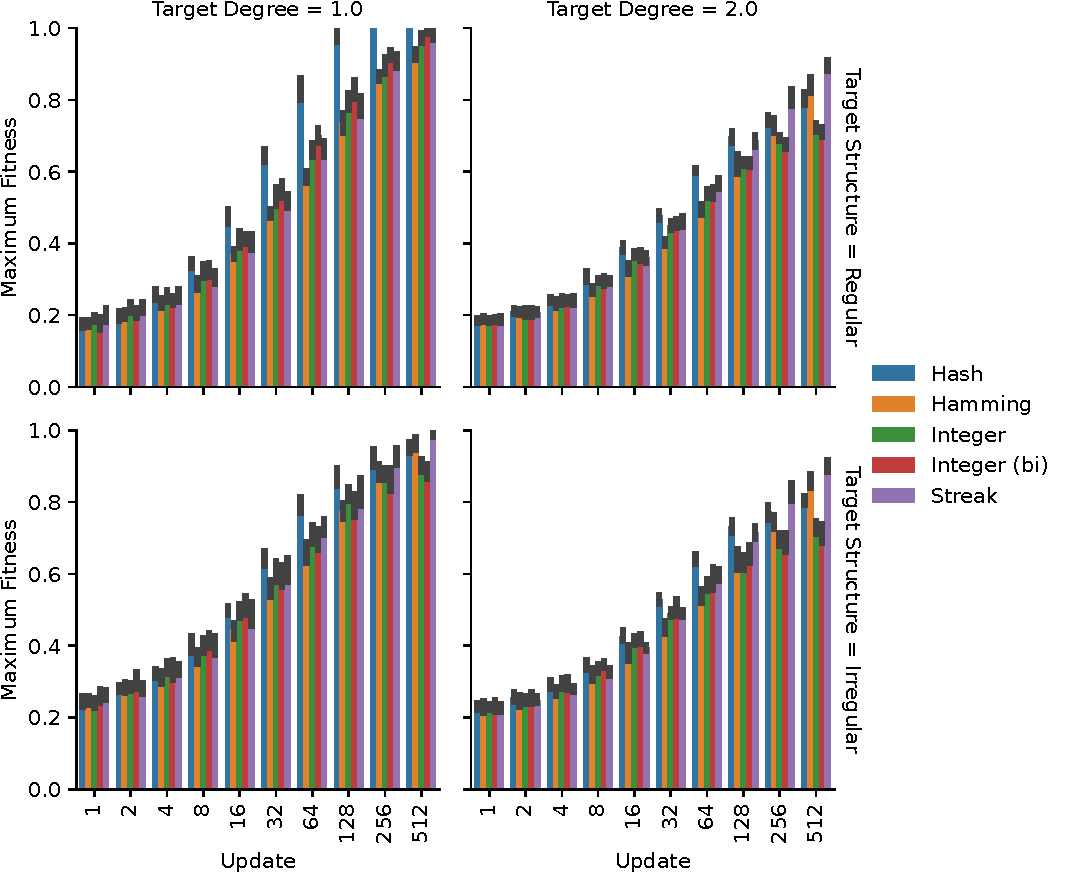
\includegraphics[width=0.75\textwidth]{img/target_evolve_big/viz=max-fitness-bar+_data_hathash_hash=fec9ab60c905d6fd+_script_fullcat_hash=c26c8688c31571c2+ext=}
\end{minipage}
\begin{minipage}{6in}
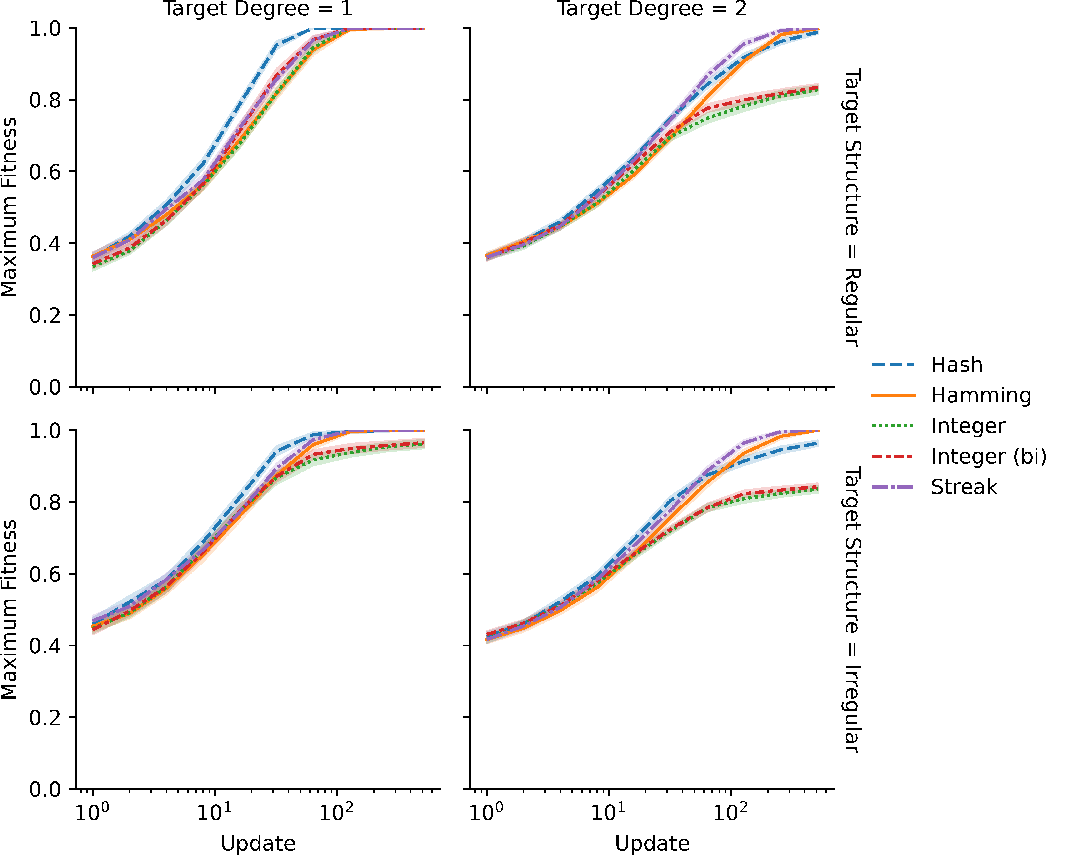
\includegraphics[width=0.75\textwidth]{img/target_evolve/viz=max-fitness-line+_data_hathash_hash=673d309ab90e91d1+_script_fullcat_hash=c152ead38b1c5ffb+ext=}
\end{minipage}
\begin{minipage}{\textwidth}
\caption{
Trajectories of adaptive evolution for each tag-matching metric on the 64-node graph-matching task.
Maximum fitness is the best fitness value for any individual within a population.
Reported results use each metric's best-performing per-bit mutation rate.
(See Supplementary Figure \ref{fig:evolve_big_mutsweep} for survey showing how mutation rate affects adaptive evolution under each metric.)
Note log-scale x-axes.
Shaded area and error bars represent bootstrapped 95\% confidence intervals across 10 replicate observations.
}
\label{fig:evolve_bests64}
\end{minipage}
\end{figure*}
